\chapter{Foundations of Probability}
\label{ch:foundations}

% --- Section: Intuition ---
\section{Probability and Intuition}

Sometimes our intuition misleads us. To be more accurate, we need to recognize that intuition can be wrong for mainly two reasons:

\begin{enumerate}
    \item Misunderstanding the terminology of the problem.
    \item Biases from past experiences.
\end{enumerate}

\begin{intuition}
Intuition about probability often fails because our minds rely on past experience or oversimplified reasoning. Being aware of this can help us approach problems more carefully.
\end{intuition}

\begin{problem}
Consider the following statements. Decide whether they are true or false, and explain why.
\end{problem}

\begin{eg}[Fair Coin Toss]
\textbf{Statement:} When we toss a fair coin, the chance of heads is $\frac{1}{2}$ and the chance of tails is $\frac{1}{2}$.  

\textbf{Answer:} True. This is the definition of a fair coin.
\end{eg}

\begin{eg}[Possible Outcomes]
\textbf{Statement:} When we toss a coin, there are 2 possible outcomes: H or T.  

\textbf{Answer:} Mostly true, but it depends on the experiment's definition. What if the coin lands on its edge? We typically simplify the model to include only Heads and Tails.
\end{eg}

\begin{eg}[Mean vs. Median]
\textbf{Statement:} We have a set of 1000 numbers. Their average is $A$. Half the numbers are $\leq A$, and half are $> A$.  

\textbf{Answer:} False. This describes the \textbf{median}, not the \textbf{average} (mean). Consider the set $\{1, 2, 97\}$. The average is $A=33.3$, but two-thirds of the numbers are less than $A$.
\end{eg}

\begin{eg}[Random Number Probability]
\textbf{Statement:} I will randomly pick a number from $\{1, 2, 3, 4\}$. What is $P(1)$?  

\textbf{Answer:} It is $\frac{1}{4}$, but only if "randomly" implies that each outcome is equally likely (a uniform distribution). The term "random" alone is not sufficient.
\end{eg}

\begin{eg}[Average Number of Legs]
\textbf{Statement:} What are the chances that the next person who walks into this room has more than the average number of legs?  

\textbf{Answer:} Extremely high (close to 100\%). The vast majority of people have two legs. A very small number of people have one or zero legs. The average number of legs for a human population will be slightly less than 2 (e.g., 1.999...). Therefore, almost everyone has more than the average.
\end{eg}

\begin{remark}
Always clarify definitions and assumptions in probability problems. \\
Words like "random" or "average" can be misleading if interpreted naively.
\end{remark}
% --- Section: Experiments and Sample Spaces ---
\section{Random Experiments and Sample Spaces}

To formalize probability, we begin with a few core definitions.

\begin{definition}[Random Experiment]
A well-defined procedure that results in an uncertain outcome.
\end{definition}

\begin{definition}[Outcome]
A single result of a random experiment.
\end{definition}

\begin{definition}[Sample Space]
The set of all possible outcomes of a random experiment, denoted $S$.
\end{definition}

\begin{definition}[Trial]
Each attempt or performance of a random experiment is called a trial.
\end{definition}

\begin{definition}[Event]
Any subset of the sample space ($A \subseteq S$). An event is a set of outcomes.
\end{definition}

\begin{remark}
The most critical step in solving a probability problem is often defining the sample space correctly. A poorly defined sample space can lead to incorrect probability calculations.
\end{remark}

\begin{eg}[Examples of Sample Spaces]
Here are several random experiments and their corresponding sample spaces:

\begin{description}
    \item[$E_1$:] Roll a fair die and record the top face. \\
    $S_1 = \{1, 2, 3, 4, 5, 6\}$

    \item[$E_2$:] Toss a coin twice and record the sequence of outcomes. \\
    $S_2 = \{HH, HT, TH, TT\}$

    \item[$E_3$:] Toss a die twice and record the sum of the faces. \\
    $S_3 = \{2, 3, \dots, 12\}$

    \item[$E_4$:] Toss a 3-sided die twice and record the ordered pair of results. \\
    $S_4 = \{(i,j) : i,j \in \{1,2,3\}\} = \{(1,1), (1,2), (1,3), (2,1), \dots, (3,3)\}$

    \item[$E_5$:] Toss a 3-sided die twice and record the set of results (order ignored). \\
    $S_5 = \{\{i,j\} : i,j \in \{1,2,3\}\} = \{\{1,1\}, \{1,2\}, \{1,3\}, \{2,2\}, \{2,3\}, \{3,3\}\}$

    \item[$E_6$:] Toss a coin until the first head appears, recording the number of tosses. \\
    $S_6 = \{1, 2, 3, \dots \} = \mathbb{N}^+$

    \item[$E_7$:] Pick a random English word and record its number of letters. \\
    $S_7 = \{1, 2, 3, \dots \}$
\end{description}
\end{eg}
% --- Section: Probability Measures ---
\section{Probability Measures}

A probability measure (or probability distribution) is a function that assigns a likelihood to each event.

\begin{definition}[Probability Measure]
A probability measure is a function 
\[
P: \mathcal{P}(S) \to [0,1]
\] 
that maps events in the sample space $S$ to a real number between 0 and 1. It must satisfy the following three axioms:
\begin{enumerate}
    \item \textbf{Non-negativity:} For any event $A \subseteq S$, $P(A) \geq 0$.
    \item \textbf{Normalization:} The probability of the entire sample space is 1, i.e., $P(S) = 1$.
    \item \textbf{Additivity:} For any finite collection of pairwise disjoint events. \\ 
    $$A_1, A_2, \dots, A_n$$ (meaning $A_i \cap A_j = \emptyset$ for $i \neq j$), \\ 
    the probability of their union is the sum of their individual probabilities:
    \[
        P\left(\bigcup_{i=1}^{n} A_i\right) = \sum_{i=1}^{n} P(A_i).
    \]
\end{enumerate}
\end{definition}

\begin{remark}
Intuitively, a probability measure quantifies how likely an event is to occur. The axioms ensure probabilities are consistent: they cannot be negative, the total probability is 1, and disjoint events’ probabilities add up.
\end{remark}
% --- Section: Computing Probabilities ---
\section{Computing Probabilities}

Let's apply the concepts of probability measures to compute probabilities in various scenarios.

\begin{eg}[Fair 12-sided Die]
Throw a fair 12-sided die. The sample space is $S = \{1, 2, \dots, 12\}$. Each outcome has probability $\frac{1}{12}$. Let $E$ be the event of rolling an even number and $F$ be the event of rolling a number $\le 4$:
\[
    E = \{2, 4, 6, 8, 10, 12\}, \quad F = \{1, 2, 3, 4\}.
\]
The probabilities are:
\begin{itemize}
    \item $P(E) = \frac{|E|}{|S|} = \frac{6}{12} = \frac{1}{2}$
    \item $P(F) = \frac{|F|}{|S|} = \frac{4}{12} = \frac{1}{3}$
    \item $P(E \cap F) = P(\{2,4\}) = \frac{2}{12} = \frac{1}{6}$
    \item $P(F^c) = 1 - P(F) = 1 - \frac{1}{3} = \frac{2}{3}$
\end{itemize}
\end{eg}

\begin{eg}[Sum of Two Dice]
Throw a fair 6-sided die twice and record the sum. The sample space of ordered pairs is $S' = \{(i,j) : i,j \in \{1,\dots,6\}\}$, so $|S'| = 36$. The sample space for the sum is $S = \{2, 3, \dots, 12\}$. Outcomes in $S$ are not equally likely. Let $E$ be the event that the sum is even.
\[
P(\text{Sum}=2) = \frac{1}{36}, \quad 
P(\text{Sum}=3) = \frac{2}{36}, \quad 
P(\text{Sum}=4) = \frac{3}{36}.
\]

\begin{center}
\begin{tabular}{lcccccc}
\toprule
Sum & 2 & 4 & 6 & 8 & 10 & 12 \\
\midrule
\# Ways & 1 & 3 & 5 & 5 & 3 & 1 \\
\bottomrule
\end{tabular}
\end{center}

So, 
\[
P(E) = \frac{1+3+5+5+3+1}{36} = \frac{18}{36} = \frac{1}{2}.
\]
\end{eg}

\begin{eg}[Weighted Die]
Consider a 5-sided die where $P(k) = c \cdot k$. Using normalization $\sum_{k=1}^{5} P(k) = 1$:
\[
c(1+2+3+4+5) = 15c = 1 \implies c = \frac{1}{15}.
\]
Then $P(k) = \frac{k}{15}$. The probability of rolling an even face is
\[
P(\text{even}) = P(\{2,4\}) = \frac{2}{15} + \frac{4}{15} = \frac{6}{15} = \frac{2}{5}.
\]
\end{eg}

\begin{eg}[Permutations]
Consider all permutations of $\{1,2,3\}$ with equal probability. Let $E$ be "starts with 1" and $F$ be "2 comes before 3":
\[
E = \{123, 132\} \implies P(E) = \frac{2}{6} = \frac{1}{3}, \quad 
F = \{123, 213, 231\} \implies P(F) = \frac{3}{6} = \frac{1}{2}.
\]
\end{eg}

\begin{eg}[Weighted Permutations]
Consider permutations of $\{1,2,3,4\}$. Let $P(abcd) \propto a$, the first element. Sum of weights: \\ 
$6(1)+6(2)+6(3)+6(4) = 60 \implies P(x) = \frac{a}{60}$.  

Let $E = \{abcd \in S_4 \mid a<b \text{ and } c<d\} = \{1234, 1324, 1423, 2314, 2413, 3412\}$. Then
\[
P(E) = \frac{1+1+1+2+2+3}{60} = \frac{10}{60} = \frac{1}{6}.
\]
\end{eg}

\begin{remark}
Weighted probabilities allow modeling biased or non-uniform scenarios. Always normalize probabilities to ensure the total sum equals 1.
\end{remark}
% --- Section: Conditional Probability ---
\section{Conditional Probability}

Conditional probability measures the likelihood of an event occurring given that another event has already occurred. It is a fundamental concept that allows us to update our beliefs in light of new evidence.

\begin{definition}[Conditional Probability]
Given two events $A$ and $B$ from a sample space $S$, with $P(B) > 0$, the \textbf{conditional probability of $A$ given $B$} is defined as:
\[
    P(A|B) = \frac{P(A \cap B)}{P(B)}.
\]
This formula re-scales the probability of the intersection of $A$ and $B$ by the probability of the given event, $B$. In essence, we are treating $B$ as our new, smaller sample space.
\end{definition}

\begin{eg}[Medical Testing]
Consider a medical test for a disease. Let $S$ be the event that a person has the disease, and $\bar{S}$ the event they do not. Let \texttt{pos} and \texttt{neg} denote positive and negative test results, respectively.

We are given:
\begin{itemize}
    \item The probability of having the disease (prevalence): $P(S) = 0.20$ ($P(\bar{S}) = 0.80$).
    \item Probability of a positive test if the patient has the disease (sensitivity): $P(\text{pos}|S) = 0.97$.
    \item Probability of a negative test if the patient does not have the disease (specificity): $P(\text{neg}|\bar{S}) = 0.90$.
\end{itemize}

From these, we deduce:
\begin{itemize}
    \item False Negative Rate: $P(\text{neg}|S) = 1 - 0.97 = 0.03$.
    \item False Positive Rate: $P(\text{pos}|\bar{S}) = 1 - 0.90 = 0.10$.
\end{itemize}

\paragraph{Step 1: Compute Joint Probabilities}
Using the multiplication rule $P(A \cap B) = P(B) P(A|B)$:
\begin{align*}
    P(S \cap \text{pos}) &= 0.20 \times 0.97 = 0.194, \\
    P(S \cap \text{neg}) &= 0.20 \times 0.03 = 0.006, \\
    P(\bar{S} \cap \text{pos}) &= 0.80 \times 0.10 = 0.080, \\
    P(\bar{S} \cap \text{neg}) &= 0.80 \times 0.90 = 0.720.
\end{align*}

\begin{figure}[H]
    \centering
    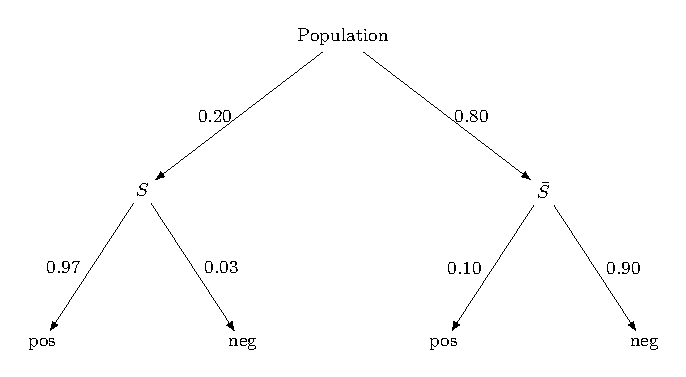
\includegraphics[width=0.7\textwidth]{figures/tree_medicalTesting.pdf}
    \caption{Tree diagram illustrating the relationships between disease status and test results.}
    \label{fig:tree_medical_testing}
\end{figure}

\paragraph{Step 2: Compute the Marginal Probability of a Positive Test}
\[
    P(\text{pos}) = P(S \cap \text{pos}) + P(\bar{S} \cap \text{pos}) = 0.194 + 0.080 = 0.274.
\]

\paragraph{Step 3: Compute the Posterior Probability}
\[
    P(S|\text{pos}) = \frac{P(S \cap \text{pos})}{P(\text{pos})} = \frac{0.194}{0.274} \approx 0.708.
\]

\begin{intuition}[Understanding Bayes' Theorem]
Even with a highly accurate test, a positive result does not guarantee the presence of the disease. This is because the overall prevalence of the disease in the population affects the probability. Bayes' theorem allows us to "update" our belief by combining the test's accuracy with prior information (prevalence).
\end{intuition}
\end{eg}


\begin{eg}[Blood Type Distribution]
The joint probability distribution \( P(\text{Type} \cap \text{Category}) \) for individuals classified by blood type and category (P, Q, R, S, T) is given in Table~\ref{tab:bloodtype}.

\begin{table}[H]
    \centering
    \begin{tabular}{l|ccccc}
        \toprule
        \textbf{Blood Type} & \textbf{P} & \textbf{Q} & \textbf{R} & \textbf{S} & \textbf{T} \\
        \midrule
        A  & 0.30 & 0.40 & 0.20 & 0.45 & 0.20 \\
        B  & 0.30 & 0.30 & 0.10 & 0.45 & 0.20 \\
        AB & 0.20 & 0.10 & 0.40 & 0.05 & 0.30 \\
        O  & 0.20 & 0.20 & 0.30 & 0.05 & 0.30 \\
        \bottomrule
    \end{tabular}
    \caption{Rescaled joint distribution where each category column sums to 1.}
    \label{tab:bloodtype}
\end{table}

\paragraph{(a) Probability of blood type A given category T}
\[
P(A \mid T) = \frac{P(A \cap T)}{P(T)} = \frac{0.20}{1.00} = 0.20.
\]

\paragraph{(b) Probability of blood type B given category Q}
\[
P(B \mid Q) = \frac{P(B \cap Q)}{P(Q)} = \frac{0.30}{1.00} = 0.30.
\]

\paragraph{(c) Probability of blood type A or B given category Q}
\[
P((A \cup B) \mid Q) = \frac{P(A \cap Q) + P(B \cap Q)}{P(Q)} 
= \frac{0.40 + 0.30}{1.00} = 0.70.
\]
\end{eg}

\begin{remark}
Conditional probability allows reasoning about events under additional information. Tree diagrams and tables are effective tools for visualizing and computing these probabilities.
\end{remark}
% --- Section: Independence of Events ---
\section{Independence of Events}

\subsection{Joint Probability}
For any two events $A$ and $B$, the general rule is:
\[
P(A \cap B) \neq P(A) \cdot P(B)
\]

However, there is an important exception: if events $A$ and $B$ are independent, then
\[
P(A \cap B) = P(A) \cdot P(B).
\]

\begin{explanation}
This multiplication rule applies only when the events do not influence each other.
\end{explanation}

\subsection{Definition of Independence}
\begin{definition}[Independence]
Events $A$ and $B$ are said to be \textbf{independent} if and only if:
\[
P(A \cap B) = P(A) \cdot P(B)
\]
\end{definition}

\begin{explanation}
Knowing the outcome of event $A$ provides no information about the likelihood of event $B$, and vice versa.
\end{explanation}

\subsection{Example 1: Fair Die Tosses}

\begin{eg}
Consider tossing a fair 6-sided die twice. We want to find the probability that:

\[
\text{the first face shows a ``2'' and the second face is odd.}
\]

Since the two tosses are independent, we can apply the \textbf{multiplication rule}:

\[
\begin{aligned}
P(\text{first face = 2 and second face odd}) 
&= P(\text{first face = 2}) \cdot P(\text{second face odd}) \\
&= \frac{1}{6} \cdot \frac{3}{6} \\
&= \frac{1}{12}.
\end{aligned}
\]

Therefore, the probability is:

\[
\frac{1}{12} \approx 0.0833 \text{ or } 8.33\%.
\]
\end{eg}

\subsection{Example 2: Testing Independence Numerically}
\begin{eg}[Population Data]
Consider selecting a Moroccan person at random:

\begin{itemize}
    \item $A$: person is female
    \item $B$: person is a nurse
    \item $C$: person is a school teacher
\end{itemize}

\paragraph{Given Data:}
\[
P(A) = 0.50, \quad P(B) = 0.05, \quad P(C) = 0.01
\]
\[
\text{80\% of nurses are women, 50\% of school teachers are women.}
\]

\paragraph{Step 1: Check $A$ and $B$}
\[
P(A \cap B) = 0.80 \times 0.05 = 0.04, \quad P(A) \cdot P(B) = 0.50 \times 0.05 = 0.025
\]

\begin{observe}
Since $0.04 \neq 0.025$, $A$ and $B$ are \textbf{not independent}.
\end{observe}

\paragraph{Step 2: Check $A$ and $C$}
\[
P(A \cap C) = 0.50 \times 0.01 = 0.005, \quad P(A) \cdot P(C) = 0.50 \times 0.01 = 0.005
\]

\begin{observe}
Since $0.005 = 0.005$, $A$ and $C$ \textbf{are independent}.
\end{observe}
\end{eg}

\begin{intuition}[Independence Intuition]
Two events are independent if knowing one occurs does not change the probability of the other. Numerical checks reveal hidden correlations or biases.
\end{intuition}

\subsection{Union of Two Events}
\begin{definition}[Union of Events]
For events $A$ and $B$, the union $A \cup B$ represents the event that at least one of $A$ or $B$ occurs:
\[
P(A \cup B) = P(A) + P(B) - P(A \cap B)
\]
\end{definition}

\begin{explanation}
This is the principle of inclusion--exclusion: subtract the intersection so that outcomes are not double-counted.
\end{explanation}

\subsection{Example: Students at AUI}
\begin{eg}[Sports Participation]
A university has $3500$ students. The distribution of sports is:

\begin{itemize}
    \item $800$ students play football ($F$)
    \item $300$ students swim ($S$)
    \item $120$ students do both
\end{itemize}

\subsubsection*{Step 0: Visual Representation}
\begin{figure}[H]
    \centering
    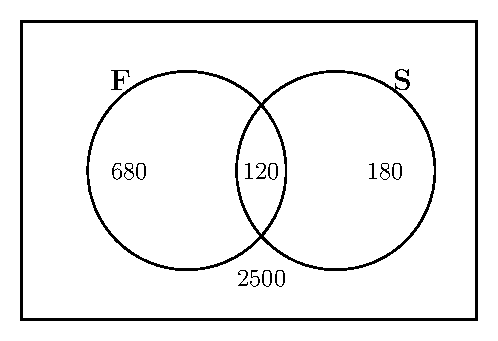
\includegraphics[width=0.7\textwidth]{figures/venn_conditional.pdf}
    \caption{Venn diagram showing football ($F$) and swimming ($S$) students at AUI.}
    \label{fig:venn_football_swim}
\end{figure}

\subsubsection*{Step a) Probability student plays football}
\[
P(F) = \frac{800}{3500} = \frac{8}{35}
\]

\subsubsection*{Step b) Probability student swims}
\[
P(S) = \frac{300}{3500} = \frac{3}{35}
\]

\subsubsection*{Step c) Probability student plays both football and swimming}
\[
P(F \cap S) = \frac{120}{3500} = \frac{6}{175}
\]

\subsubsection*{Step d) Probability student plays football or swims}
\[
P(F \cup S) = P(F) + P(S) - P(F \cap S) = \frac{7}{25}
\]

\subsubsection*{Step e) Probability student plays football given that they swim}
\[
P(F \mid S) = \frac{P(F \cap S)}{P(S)} = \frac{2}{5}
\]

\subsubsection*{Step f) Probability student plays football given that they do \textbf{not} swim}
\[
P(F \cap S^c) = P(F) - P(F \cap S) = \frac{34}{175}, \quad P(S^c) = 1 - P(S) = \frac{32}{35}
\]
\[
P(F \mid S^c) = \frac{P(F \cap S^c)}{P(S^c)} = \frac{17}{80}
\]

\subsubsection*{Step g) Probability student plays neither football nor swimming}
\[
P(F^c \cap S^c) = 1 - P(F \cup S) = \frac{18}{25}
\]

\subsubsection*{Step h) Probability student plays both football and swimming given they play at least one}
\[
P(F \cap S \mid F \cup S) = \frac{6}{49}
\]
\end{eg}

\begin{remark}
Conditional and joint probabilities, combined with independence checks, allow us to solve real-life problems such as sports participation by properly counting overlapping events.
\end{remark}

\section{Venn Diagram Probability Problems}

\subsection{Three-Set Venn Diagram}
\begin{definition}[Venn Diagram for Three Sets]
A Venn diagram represents three sets $A$, $B$, and $C$ and their relationships, including all possible intersections and complements. It is a visual tool to solve probability problems involving unions, intersections, and conditional probabilities.
\end{definition}

\begin{figure}[H]
    \centering
    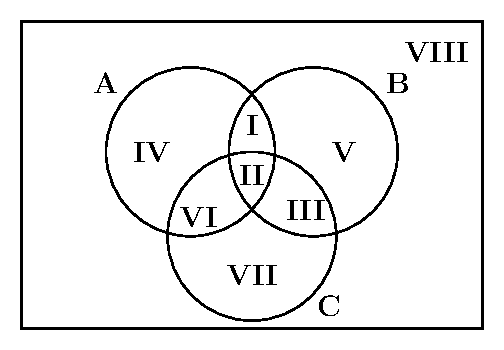
\includegraphics[width=0.6\textwidth]{figures/venn_3set.pdf}
    \caption{Three-set Venn diagram with labeled regions I--VIII.}
    \label{fig:venn3}
\end{figure}

\subsection{Region Labeling}
\begin{notation}
We assign Roman numerals I--VIII to each region in the Venn diagram as follows:
\begin{itemize}
    \item I: $A \cap B \cap C^c$ (A and B, not C)
    \item II: $A \cap B \cap C$ (all three sets)
    \item III: $A^c \cap B \cap C$ (B and C, not A)
    \item IV: $A \cap B^c \cap C^c$ (only A)
    \item V: $A^c \cap B \cap C^c$ (only B)
    \item VI: $A \cap B^c \cap C$ (A and C, not B)
    \item VII: $A^c \cap B^c \cap C$ (only C)
    \item VIII: $A^c \cap B^c \cap C^c$ (outside all sets)
\end{itemize}
\end{notation}

\subsection{Probability Solutions}
\begin{eg}[Venn Diagram Probabilities]
Let us solve the following probability problems using the labeled regions.

\paragraph{(a) Probability of $A$}
\[
P(A) = \text{I + II + IV + VI}
\]
\begin{explanation}
We sum all regions that include $A$.
\end{explanation}

\paragraph{(b) Probability of $A \cap C$}
\[
P(A \cap C) = \text{II + VI}
\]
\begin{explanation}
Only the regions that belong to both $A$ and $C$ are counted.
\end{explanation}

\paragraph{(c) Probability of $A \cup C$}
\[
P(A \cup C) = \text{I + II + III + IV + VI + VII}
\]

\paragraph{(d) Conditional Probability $P(A \mid B)$}
\[
P(A \mid B) = \frac{P(A \cap B)}{P(B)} = \frac{\text{I + II}}{\text{I + II + III + V}}
\]

\paragraph{(e) Conditional Probability $P(A \mid \overline{B \cap C})$}
\[
P(A \mid \overline{B \cap C}) = \frac{P(A \cap \overline{B \cap C})}{P(\overline{B \cap C})} = \frac{\text{I + IV + VI}}{\text{I + IV + V + VI + VII + VIII}}
\]

\paragraph{(f) Probability exactly one of $A$, $B$, or $C$ occurs}
\[
P(\text{exactly 1 of A, B, C}) = \text{IV + V + VII}
\]

\paragraph{(g) Conditional Probability $P(A \mid \overline{B} \cap C)$}
\[
P(A \mid \overline{B} \cap C) = \frac{P(A \cap \overline{B} \cap C)}{P(\overline{B} \cap C)} = \frac{\text{VI}}{\text{VI + VII}}
\]

\paragraph{(h) Conditional Probability of only $A$ given $A \cup B$}
\[
P(\text{only A} \mid A \cup B) = \frac{P(\text{only A})}{P(A \cup B)} = \frac{\text{IV}}{\text{I + II + III + IV + V + VI}}
\]

\begin{intuition}[Venn Diagram Approach]
Labeling regions helps systematically account for overlapping areas. By referring to regions with Roman numerals, we avoid double-counting and make conditional probabilities clear.
\end{intuition}

\end{eg}

\section{Important Probability Theorems}

\subsection{Total Probability Theorem}

\begin{theorem}[Total Probability Theorem]
Let $\{B_1, B_2, \ldots, B_n\}$ form a partition of the sample space $S$ (i.e., mutually exclusive and exhaustive). Then for any event $A$:
\[
P(A) = \sum_{i=1}^{n} P(A \mid B_i) \cdot P(B_i)
\]
\end{theorem}

\begin{proof}
Since $\{B_1, B_2, \ldots, B_n\}$ is a partition of $S$, we have
\[
A = A \cap S = A \cap \bigcup_{i=1}^{n} B_i = \bigcup_{i=1}^{n} (A \cap B_i)
\]
where the sets $A \cap B_i$ are mutually exclusive. By the \textbf{additivity of probability}:
\[
P(A) = \sum_{i=1}^{n} P(A \cap B_i)
\]
Using the definition of conditional probability, $P(A \cap B_i) = P(A \mid B_i) \cdot P(B_i)$. Substituting gives:
\[
P(A) = \sum_{i=1}^{n} P(A \mid B_i) \cdot P(B_i)
\]
\end{proof}

\begin{explanation}
The theorem allows us to compute the probability of $A$ by considering all “paths” $B_i$ through which $A$ can occur, then summing their contributions.
\end{explanation}

\begin{eg}[Special Case: Two Events]
For $B$ and its complement $B^c$:
\[
P(A) = P(A \mid B) \cdot P(B) + P(A \mid B^c) \cdot P(B^c)
\]
\end{eg}

\begin{eg}[Venn Diagram Example]
Using labeled Venn diagram regions:
\[
P(A) = \frac{\text{I + II}}{\text{I + II + III + V}} \cdot P(B) + \frac{\text{IV + VI}}{\text{IV + VI + VII + VIII}} \cdot P(B^c)
\]
\end{eg}

\begin{intuition}[Understanding Total Probability]
Think of the partition as splitting the sample space into mutually exclusive “paths” through which event $A$ can occur. Summing the contributions gives the total probability of $A$.
\end{intuition}

\subsection{Bayes' Theorem}

\begin{theorem}[Bayes' Theorem]
For any events $A$ and $B$ with $P(A) > 0$:
\[
P(B \mid A) = \frac{P(A \mid B) \cdot P(B)}{P(A)}
\]
\end{theorem}

\begin{proof}
By the definition of conditional probability:
\[
P(B \mid A) = \frac{P(B \cap A)}{P(A)} = \frac{P(A \cap B)}{P(A)}
\]
Using the definition of conditional probability again, $P(A \cap B) = P(A \mid B) \cdot P(B)$. Substituting gives:
\[
P(B \mid A) = \frac{P(A \mid B) \cdot P(B)}{P(A)}
\]
\end{proof}

\begin{explanation}
Bayes’ Theorem updates our belief about $B$ after observing $A$. It “flips” conditional probabilities, weighting by the prior probability of $B$.
\end{explanation}

\begin{eg}[Using Total Probability in Bayes]
If $\{B, B^c\}$ is a partition:
\[
P(B \mid A) = \frac{P(A \mid B) \cdot P(B)}{P(A \mid B) \cdot P(B) + P(A \mid B^c) \cdot P(B^c)}
\]
\end{eg}

\begin{eg}[General Partition]
For a partition $\{B_1, \ldots, B_n\}$:
\[
P(B_i \mid A) = \frac{P(A \mid B_i) \cdot P(B_i)}{\sum_{j=1}^{n} P(A \mid B_j) \cdot P(B_j)}
\]
\end{eg}

\begin{eg}[Venn Diagram Interpretation]
Using Venn diagram regions:
\[
P(B \mid A) = \frac{P(A \cap B)}{P(A)} = \frac{\text{I + II}}{\text{I + II + IV + VI}}
\]
\end{eg}

\begin{intuition}[Bayes Intuition]
Bayes’ Theorem allows us to answer: “Given we observed $A$, what is the probability that $B$ occurred?” It converts prior knowledge and likelihoods into updated beliefs.
\end{intuition}
